\documentclass[problem]{mcs}

\begin{pcomments}
  \pcomment{PS_tangled_and_mangled_graphs}
  \pcomment{from: S08.ps5; parts reordered 10/16/09 by ARM}
\end{pcomments}

\pkeywords{
  connected
  tangled_graph
  mangled_graph
  buildup_error
}

%%%%%%%%%%%%%%%%%%%%%%%%%%%%%%%%%%%%%%%%%%%%%%%%%%%%%%%%%%%%%%%%%%%%%
% Problem starts here
%%%%%%%%%%%%%%%%%%%%%%%%%%%%%%%%%%%%%%%%%%%%%%%%%%%%%%%%%%%%%%%%%%%%%

\begin{problem}
An edge is said to \emph{leave} a set of vertices if one end of the edge
is in the set and the other end is not.

\bparts

\problempart An $n$-node graph is said to be \term*{mangled} if there is
an edge leaving every set of $\floor{n/2}$ or fewer vertices.
Prove the following claim.

\begin{claim*}
  Every mangled graph is connected.
\end{claim*}

\begin{solution}
  The proof is by contradiction.  Assume for the purpose of contradiction
  that these exists an $n$-node graph that is mangled, but not connected.
  Then the graph must have at least two connected components.  However,
  there can be at most one connected component of size more than
  $\floor{n/2}$, since $2\paren{\floor{n/2} +1} > n$.  Therefore, there
  exists a connected component with $\floor{n/2}$ or fewer vertices.
  Since the graph is mangled, there is an edge leaving this component.
  But this contradicts the definition of a connected component.
\end{solution}

\eparts

An $n$-node graph is said to be {\em tangled} if there is an edge leaving
every set of $\ceil{n/3}$ or fewer vertices.

\bparts

\problempart\label{tanglenotconn} Draw a tangled graph that is not connected.

\begin{solution} A tangled but non-connected graph is the following:
\begin{center}
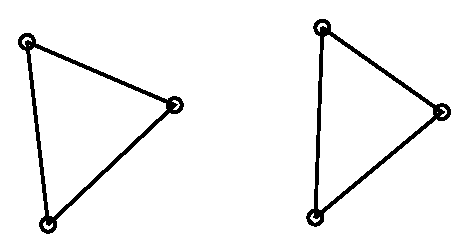
\includegraphics[width=1.0in]{figures/ps3-tangled-cx}
\end{center}
\end{solution}

\problempart Find the error in the proof of the following

\begin{falseclm*}
Every tangled graph is connected.
\begin{falseproof}

The proof is by strong induction on the number of vertices in the graph.
Let $P(n)$ be the proposition that if an $n$-node graph is tangled, then
it is connected.  In the base case, $P(1)$ is true because the graph
consisting of a single node is trivially connected.

For the inductive case, assume $n \geq 1$ and $P(1), \ldots, P(n)$ hold.
We must prove $P(n+1)$, namely, that if an $(n+1)$-node
graph is tangled, then it is connected.

So let $G$ be a tangled, $(n+1)$-node graph.  Choose $\ceil{n/3}$ of the
vertices and let $G_1$ be the tangled subgraph of $G$ with these vertices
and $G_2$ be the tangled subgraph with the rest of the vertices.  Note
that since $n \geq 1$, the graph $G$ has a least two vertices, and so both
$G_1$ and $G_2$ contain at least one vertex.  Since $G_1$ and $G_2$ are
tangled, we may assume by strong induction that both are connected.  Also,
since $G$ is tangled, there is an edge leaving the vertices of $G_1$ which
necessarily connects to a vertex of $G_2$.  This means there is a path
between any two vertices of $G$: a path within one subgraph if both
vertices are in the same subgraph, and a path traversing the connecting
edge if the vertices are in separate subgraphs.  Therefore, the entire
graph, $G$, is connected.  This completes the proof of the inductive case,
and the Claim follows by strong induction.

\end{falseproof}
\end{falseclm*}

\begin{solution}
  The error is in the statement, ``Let $G_1$ be the \emph{tangled}
  subgraph \dots.''  This makes the implicit assumption that a tangled
  graph can be split into tangled subgraphs, one of which is of size at
  most $\ceil{n/3}$.  This assumption is false. To see why, consider the
  counterexample given in part~\eqref{tanglenotconn}.  That graph is
  tangled and $\ceil{n/3}=2$.  But, no matter how we split the graph into
  two subgraphs of sizes either 2~and~4 or 1~and~5, one of the two is not
  tangled.

  It's a common blunder to assume that a property of a graph is
  ``inherited'' by a subgraph.  This is true for many familiar properties
  such as being $k$-colorable, having degrees bounded by a constant $d$,
  being planar, being no larger than the whole graph.  But many other
  familiar are not inherited, for example, being a tree, being a simple
  cycle, requiring more than $k$ colors, being nonplanar.
\end{solution}

\eparts

\end{problem}

%%%%%%%%%%%%%%%%%%%%%%%%%%%%%%%%%%%%%%%%%%%%%%%%%%%%%%%%%%%%%%%%%%%%%
% Problem ends here
%%%%%%%%%%%%%%%%%%%%%%%%%%%%%%%%%%%%%%%%%%%%%%%%%%%%%%%%%%%%%%%%%%%%%
\endinput
